\documentclass[12pt, a4paper]{book}

\usepackage{fancyhdr}
\usepackage[left=4cm, right=4cm, top=4cm, bottom=4cm]{geometry}
\usepackage[utf8]{inputenc}
\usepackage[table]{xcolor}
\usepackage{hyperref}
\usepackage{amsmath}
\usepackage{enumitem}
\usepackage{graphicx}
\usepackage{amsfonts}
\usepackage{booktabs}
\usepackage{subcaption}
\usepackage[justification=centering]{caption}
\usepackage{xepersian}

\DeclareMathOperator*{\argmax}{argmax}
\DeclareMathOperator*{\argmin}{argmin}
\newcolumntype{L}{>{$}l<{$}} % math-mode version of "l" column type

\newcommand{\coursetitle}{شبکه‌های عصبی}
\newcommand{\doctitle}{تمرین هفتم}
\newcommand{\name}{محمدرضا غفرانی}
\newcommand{\studentno}{400131076}
\newcommand{\todaydate}{\today}

\settextfont{Sahel}
\setlatintextfont{Times Newer Roman}

\pagestyle{fancy}
\lhead{\textbf{\doctitle}}
\chead{\name}
\rhead{\todaydate}

\begin{document}

\begin{flushleft}
    \name \\
    \studentno \\
    \todaydate
\end{flushleft}

\begin{center}
    \huge
    \textbf{\coursetitle}
    \break
    \large
    \doctitle
\end{center}

% suppress the fancy header on the first page only
\thispagestyle{plain}

\section*{سوال یک}

با توجه به این که شبکه \lr{GAN} از دو شبکه متفاوت تشکیل شده و هر یک از این دو شبکه‌ تابع هدف متفاوت اما
وابسته به هم دارند بنابراین آموزش این شبکه‌ها به صورت نوبتی انجام می‌شود. در یک نوبت ابتدا شبکه دسته‌بند
برای یک یا چند گام آموزش دیده و تصاویر تولید شده توسط شبکه مولد را از تصاویر واقعی جدا می‌کند. در نوبت بعد
آموزش شبکه دسته‌بند متوقف شده و آموزش شبکه مولد شروع می‌شود. شبکه مولد در این نوبت تلاش می‌کند تصاویری تولید
کند که توسط شبکه دسته‌بند قابل تفکیک از تصاویر واقعی نباشند. آموزش شبکه به این شکل ادامه پیدا کرده و در نهایت
آموزش شبکه در یک تعداد گام ثابت و یا زمانی که شبکه دسته‌بند به صورت شانسی تصاویر واقعی را از جعلی تفکیک می‌کند
متوقف می‌شود.

\section*{سوال دو}

کانولوشن عملیاتی است که لزوما حالت بازگشتی ندارد، یعنی ممکن است $y$ حاصل کانولوشن دو تابع $f$ و $g$ را باشد اما
نتوان تابع $g$ را با داشتن توابع $f$ و $y$ محاسبه کرد. دلیل این اتفاق آن است که معمولا در عمل کانولوشن چند تابع
به یک تابع تبدیل می‌شوند و در نتیجه برگشتن از تابع حاصل شده به توابع اولیه ممکن نیست.

در شبکه‌های عمیق از عمل معکوس کانولوشن برای افزایش ابعاد داده اولیه استفاده می‌شود. این عمل معکوس کانولوشن
لزوما همانند عکس تابع کانولوشن عمل نمی‌کند اما نتایج تولید شده توسط آن با ارزش است. در شکل \ref{deconvolution}
نمونه‌ای از نحوه لایه معکوس کانولوشن مشاهده می‌شود. در این جا به ورودی اصلی تعدادی حاشیه صفر اضافه می‌شود تا ابعاد
ورودی اولیه بیشتر شود. در قدم بعدی یک پنجره - همانند پنجره‌ای که در کانولوشن وجود داشت - لغزانده شده و نتیجه
نهایی تولید می‌شود.

\begin{figure}[h]
    \centering
    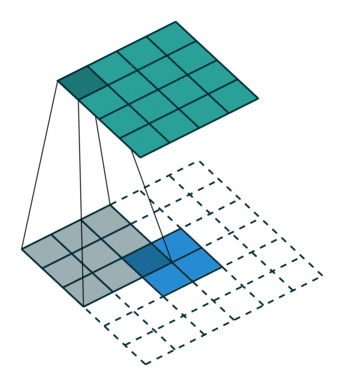
\includegraphics[scale=0.5]{images/deconvolution_step1.png}
    \caption{نحوه عملکرد معکوس کانولوشن}
    \label{deconvolution}
\end{figure}

اگر اندازه قدم در لایه معکوس کانولوشن ۲ باشد، در این حالت، برخلاف لایه کانولوشن که اندازه گام روی پنجره تاثیر گذار بود،
ورودی تحت تاثیر قرار می‌گیرد. در شکل \ref{deconvolution_step2} این حالت مشاهده می‌شود. همان‌طور که مشاهده می‌شود در این
حالت پیکسل‌های ورودی با فاصله ۲ از هم قرار گرفته‌اند و در همچنان حاشیه‌گذاری صفر روی شکل ورودی انجام شده است.

\begin{figure}
    \centering
    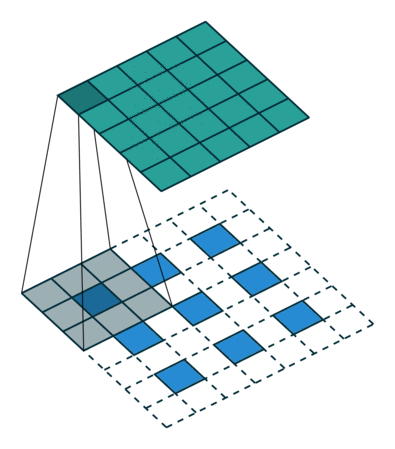
\includegraphics[scale=0.5]{images/deconvolution_step2.png}
    \caption{نحوه عملکرد معکوس کانولوشن با گام ۲}
    \label{deconvolution_step2}
\end{figure}

\clearpage

\section*{سوال سه}

تابع هزینه کلی برای شبکه \lr{GAN} به صورت زیر تعریف می‌شود.

$$\min_G \max_D \Big[\mathbb{E}_{x \sim p_{data}} \big[\log D(x)\big] + \mathbb{E}_{z \sim p_{z}(z)}\big[\log(1-D(G(z)))\big]\Big]$$

این تابع هزینه، ترکیب توابع هزینه هر دو شبکه تولیدکننده و دسته‌بند است. به عبارت ساده این تابع بیان می‌کند که
شبکه دسته‌بند باید بتواند تصاویر واقعی را برچسب واقعی و تصاویر جعلی را برچسب جعلی بزند. از طرف دیگر شبکه
تولیدکننده باید بتواند تصاویری را تولید کند که شبکه دسته‌بند را به اشتباه بیاندازد. با این توضیح می‌توانیم تابع
هزینه بالا را برای شبکه مولد به صورت زیر بازنویسی کنیم.

$$\min_G \Big[E_{z \sim p_z(z)}\big[\log(1-D(G(z)))\big]\Big]$$

از آن‌جا که تابع $\log(1-D(G(z)))$ یک تابع نسبتا هموار است بنابراین مشتق آن بسیار کم می‌شود که در نتیجه
نمی‌تواند به خوبی شبکه مولد را آموزش دهد. بنابراین این قسمت را در تابع هزینه تغییر داده و تابع هزینه شبکه
مولد را به شکل زیر بازنویسی می‌کنیم.

$$\max_G \Bigl[E_{z \sim p_z(z)}\big[\log(D(G(z)))\big]\Bigr]$$

از طرف دیگر تابع هزینه برای شبکه به صورت زیر نوشته می‌شود.

$$\max_D \Big[\mathbb{E}_{x \sim p_{data}} \big[\log D(x)\big] + \mathbb{E}_{z \sim p_{z}(z)}\big[\log(1-D(G(z)))\big]\Big]$$

پیاده‌سازی توابع بالا با استفاده از تابع هزینه \lr{cross entropy} انجام شده است.

\section*{سوال چهار}

پیش‌پردازشی که بر روی داده‌ها انجام شده است تبدیل اعداد به بازه $[0,1)$ با تقسیم آن‌ها به 255 و همچنین
تبدیل ابعاد تصاویر به $64*64$ است. این تبدیل باعث کاهش تعداد پارامتر‌های مدل و آسان‌تر شدن یادگیری می‌شود.

نتایج مربوط به تغییر تعداد لایه‌ها در مدل \lr{FCGAN} در شکل‌های \ref{fcgan_nlayer1}، \ref{fcgan_nlayer3} و
\ref{fcgan_nlayer5} آمده است. همان‌طور که مشاهده می‌شود با افزایش تعداد لایه‌های پنهان خروجی تصویر حالت
شطرنجی‌تر پیدا کرده است. دقت داشته باشید که لایه پنهان در این حالت خود متشکل از سه جز لایه متراکم، لایه نرمال‌سازی و
لایه با تابع فعال‌سازی \lr{LeakyRelu} با مقدار $\alpha=0.2$ است.
متاسفانه هیچ یک از تصاویر تولید شده شباهتی به سگ یا گربه ندارند و بنابراین نمی‌توان
بین آن‌ها تفاوت خاصی قائل شد اما با توجه به این که تصاویر تولید شده در هنگامی شبکه تعداد لایه‌های مخفی کم‌تری دارد
نرم‌تر است بنابراین می‌توان انتظار داشت که با افزایش تعداد گام‌های آموزش مدل، این شبکه‌ها نتیجه بهتری داشته باشند.

دلیل این که در حالتی که تعداد لایه‌های مخفی مدل کم‌تر است تصاویر خروجی نرم‌تر هستند را می‌توان
تعداد پارامتر‌های مدل دانست. هنگامی که تعداد پارامتر‌های مدل کم‌تر است مدل قدرت کمی در تولید تصاویر داشته و در نتیجه
بردار تصادفی ورودی را با تغییر کم‌تری خروجی می‌دهد. بنابراین تصویر تولید شده هموارتر است. اما زمانی که تعداد پارامتر‌های
مدل بیشتر است، قدرت مدل بیشتر بوده و در نتیجه ورودی را دچار تغییرات گسترده‌تری می‌کند و می‌تواند تصاویر
شطرنجی تولید کند.

\begin{figure}[h]
    \begin{subfigure}{0.3\linewidth}
        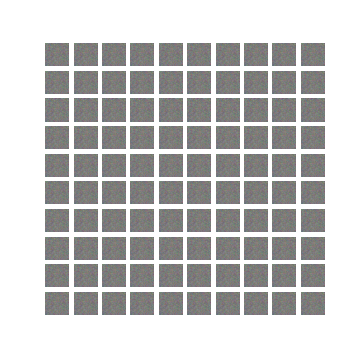
\includegraphics[width=\linewidth]{images/fcgan/nlayer1/generated_img_01.png}
        \caption{گام اول}
    \end{subfigure}
    \begin{subfigure}{0.3\linewidth}
        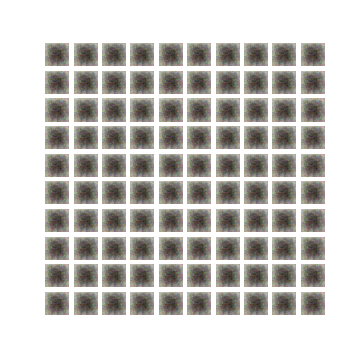
\includegraphics[width=\linewidth]{images/fcgan/nlayer1/generated_img_15.png}
        \caption{گام 15ام}
    \end{subfigure}
    \begin{subfigure}{0.3\linewidth}
        
\includegraphics[width=\linewidth]{images/fcgan/nlayer1/generated_img_30.png}
        \caption{گام 30ام}
    \end{subfigure}
    \caption{آموزش شبکه \lr{FCGAN} در طی ۳۰گام\\ تعداد لایه‌های پنهان مدل مولد=۱}
    \label{fcgan_nlayer1}
\end{figure}

\begin{figure}[h]
    \begin{subfigure}{0.3\linewidth}
        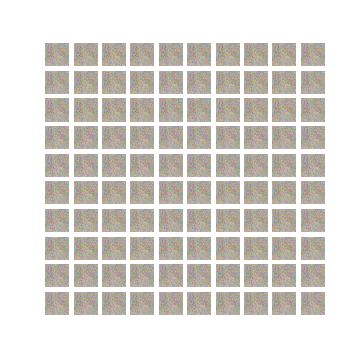
\includegraphics[width=\linewidth]{images/fcgan/nlayer3/generated_img_01.png}
        \caption{گام اول}
    \end{subfigure}
    \begin{subfigure}{0.3\linewidth}
        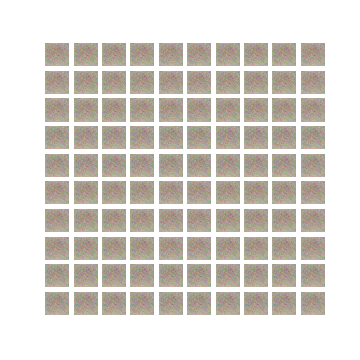
\includegraphics[width=\linewidth]{images/fcgan/nlayer3/generated_img_15.png}
        \caption{گام 15ام}
    \end{subfigure}
    \begin{subfigure}{0.3\linewidth}
        
\includegraphics[width=\linewidth]{images/fcgan/nlayer3/generated_img_30.png}
        \caption{گام 30ام}
    \end{subfigure}
    \caption{آموزش شبکه \lr{FCGAN} در طی ۳۰گام\\ تعداد لایه‌های پنهان مدل مولد=۳}
    \label{fcgan_nlayer3}
\end{figure}

\begin{figure}[h]
    \begin{subfigure}{0.3\linewidth}
        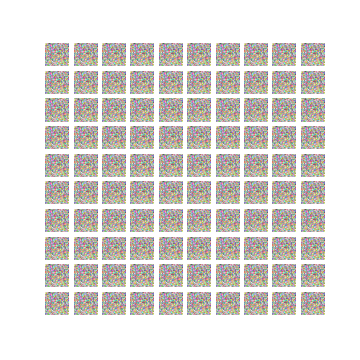
\includegraphics[width=\linewidth]{images/fcgan/nlayer5/generated_img_01.png}
        \caption{گام اول}
    \end{subfigure}
    \begin{subfigure}{0.3\linewidth}
        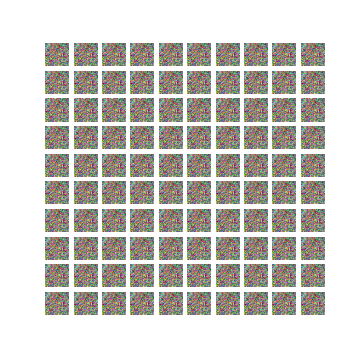
\includegraphics[width=\linewidth]{images/fcgan/nlayer5/generated_img_15.png}
        \caption{گام 15ام}
    \end{subfigure}
    \begin{subfigure}{0.3\linewidth}
        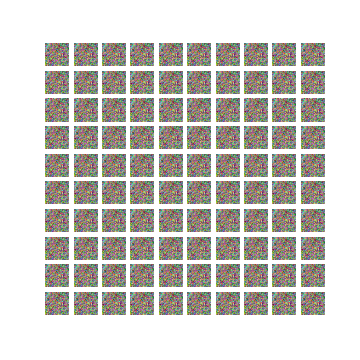
\includegraphics[width=\linewidth]{images/fcgan/nlayer5/generated_img_20.png}
        \caption{گام 30ام}
    \end{subfigure}
    \caption{آموزش شبکه \lr{FCGAN} در طی ۳۰گام\\ تعداد لایه‌های پنهان مدل مولد=5}
    \label{fcgan_nlayer5}
\end{figure}

نتایج مربوط به عملکرد مدل \lr{DCGAN} در شکل‌های \ref{dcgan_nlayer1}، \ref{dcgan_nlayer2} و \ref{dcgan_nlayer3}
آورده شده است. اولین نکته‌ای که به محض نگاه کردن به نتایج به نظر می‌رسد، بهتر بودن آن‌ها نسبت به
خروجی مدل \lr{FCGAN} است. این نکته از قبل نیز قابل پیش‌پینی بود، چرا که شبکه‌های \lr{DCGAN} حاوی
کانولوشن بوده و در نتیجه بهتر می‌توانند ویژگی‌های تصویر را استخراج و درک کنند. اما در این تصاویر نیز مشابه
خروجی شبکه \lr{FCGAN} مشابهتی با عکس سگ‌ و گربه دیده نمی‌شود.

در این حالت نیز با افزایش تعداد لایه‌های شبکه مولد خروجی تولید شده حالت شطرنجی پیدا می‌کند. به نظر می‌رسد
دلیل این حالت نیز به خاطر افزایش قدرت این شبکه‌ها باشد. در این جا نیز لایه پنهان خود متشکل از چند جز است:
لایه \lr{Conv2dTranspose} به همراه تابع فعال‌سازی \lr{LeakyRelu} با مقدار $\alpha=0.2$.

\begin{figure}[h]
    \begin{subfigure}{0.3\linewidth}
        \includegraphics[width=\linewidth]{images/dcgan/nlayer1/generated_img_01.png}
        \caption{گام اول}
    \end{subfigure}
    \begin{subfigure}{0.3\linewidth}
        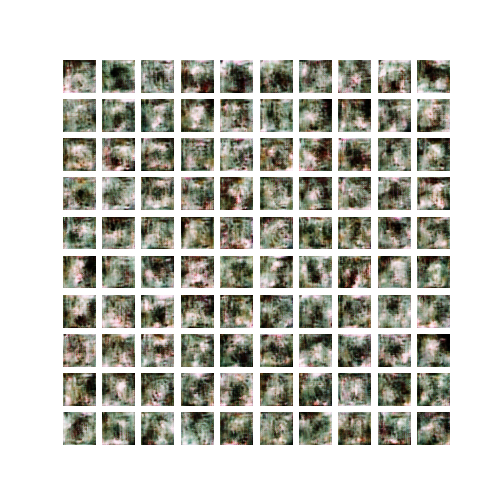
\includegraphics[width=\linewidth]{images/dcgan/nlayer1/generated_img_15.png}
        \caption{گام 15ام}
    \end{subfigure}
    \begin{subfigure}{0.3\linewidth}
        
\includegraphics[width=\linewidth]{images/dcgan/nlayer1/generated_img_30.png}
        \caption{گام 30ام}
    \end{subfigure}
    \caption{آموزش شبکه \lr{DCGAN} در طی ۳۰گام\\ تعداد لایه‌های پنهان مدل مولد=۱}
    \label{dcgan_nlayer1}
\end{figure}

\begin{figure}[h]
    \begin{subfigure}{0.3\linewidth}
        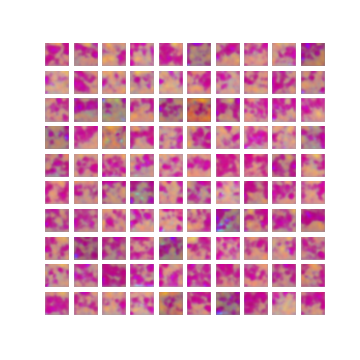
\includegraphics[width=\linewidth]{images/dcgan/nlayer2/generated_img_01.png}
        \caption{گام اول}
    \end{subfigure}
    \begin{subfigure}{0.3\linewidth}
        \includegraphics[width=\linewidth]{images/dcgan/nlayer2/generated_img_15.png}
        \caption{گام 15ام}
    \end{subfigure}
    \begin{subfigure}{0.3\linewidth}
        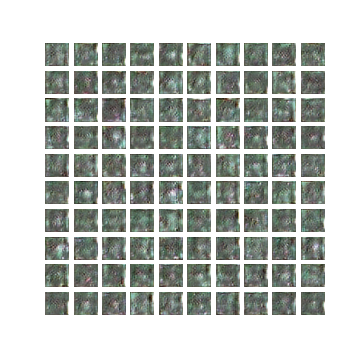
\includegraphics[width=\linewidth]{images/dcgan/nlayer2/generated_img_20.png}
        \caption{گام 30ام}
    \end{subfigure}
    \caption{آموزش شبکه \lr{DCGAN} در طی ۳۰گام\\ تعداد لایه‌های پنهان مدل مولد=2}
    \label{dcgan_nlayer2}
\end{figure}

\begin{figure}[h]
    \begin{subfigure}{0.3\linewidth}
        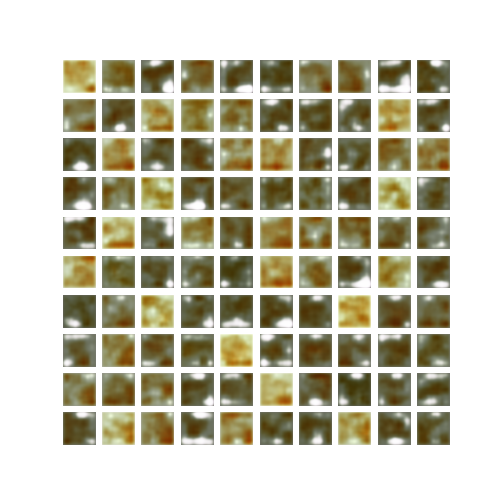
\includegraphics[width=\linewidth]{images/dcgan/nlayer3/generated_img_01.png}
        \caption{گام اول}
    \end{subfigure}
    \begin{subfigure}{0.3\linewidth}
        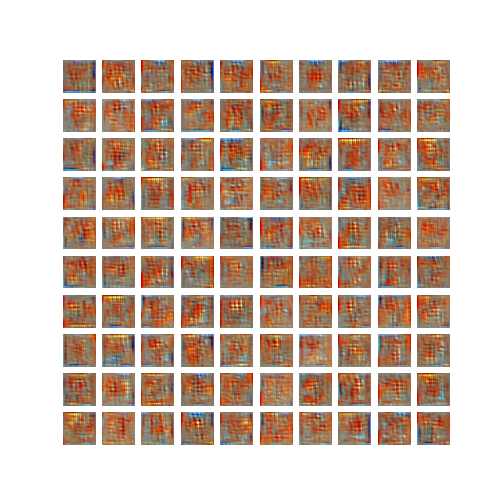
\includegraphics[width=\linewidth]{images/dcgan/nlayer3/generated_img_15.png}
        \caption{گام 15ام}
    \end{subfigure}
    \begin{subfigure}{0.3\linewidth}
        
\includegraphics[width=\linewidth]{images/dcgan/nlayer3/generated_img_30.png}
        \caption{گام 30ام}
    \end{subfigure}
    \caption{آموزش شبکه \lr{DCGAN} در طی ۳۰گام\\ تعداد لایه‌های پنهان مدل مولد=۳}
    \label{dcgan_nlayer3}
\end{figure}

تلاش‌های فراوانی برای آموزش شبکه \lr{GAN} برای تولید تصاویر با کیفیت بالا انجام شده است.
اما متاسفانه این تلاش‌ها نتیجه نداده و همان‌طور که مشاهده می‌شود خروجی‌های تولید شده از کیفیت
خوبی برخوردار نیستند. در ادامه بخشی از این تلاش‌های آورده شده است.

\begin{itemize}
    \item بررسی پیاده‌سازی مختلف موجود برای شبکه \lr{GAN}
    \item اضافه‌کردن لایه‌های \lr{Dropout} با مقدار‌های مختلف
    \item تغییر تعداد لایه‌های موجود در شبکه‌ مولد و شبکه دسته‌بند
    \item تغییر تعداد پارامتر‌های لایه‌های مختلف شبکه مولد و شبکه دسته‌بند
    \item اجازه آموزش مدل تا ۱۰۰ گام یادگیری
\end{itemize}

دلیل دیگری که به نظر می‌رسد در عدم یادگیری مدل تاثیر کلیدی داشته است، مجموعه داده انتخاب شده برای آموزش
مدل بود. با آزمایش این شبکه روی مجموعه دیگری به نام \lr{Celeb-A} که شامل تصاویر چهره اشخاص معروف است،
مشخص می‌شود که می‌توان در طی چند‌ گام به نتایج قابل قبولی رسید. چرا که در مجموعه داده \lr{Celeb-A} تصویر شامل
اجرای دیگری نیستند در حالی که در مجموعه داده \lr{cats-vs-dogs} تصاویر بعضا شامل اجرای دیگری نیز چهره انسان
نیز بوده که در نتیجه کار مدل را یادگیری سخت‌تر می‌کنند. این موضوع در شکل \ref{celeba} نیز دیده می‌شود.
همچنین لازم به ذکر است که تصویری که برای مجموعه داده \lr{Celeb-A} آورده شده است در گام پنجم آموزش است در حالی که
تصویر متناظر مجموعه داده \lr{Cats-vs-Dogs} ۳۰ گام آموزش دیده است.

\begin{figure}[h]
    \begin{subfigure}{0.4\linewidth}
        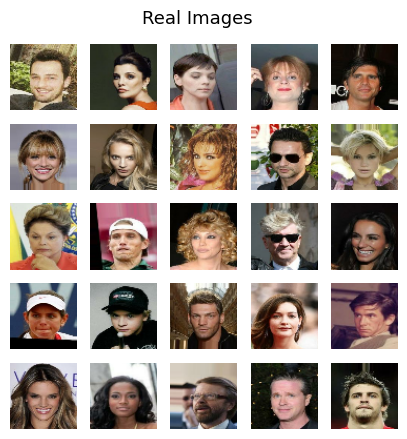
\includegraphics[width=\linewidth]{images/celeba.png}
        \caption{تصاویر مجموعه داده \lr{Celeb-A}}
    \end{subfigure}
    \hfill
    \begin{subfigure}{0.4\linewidth}
        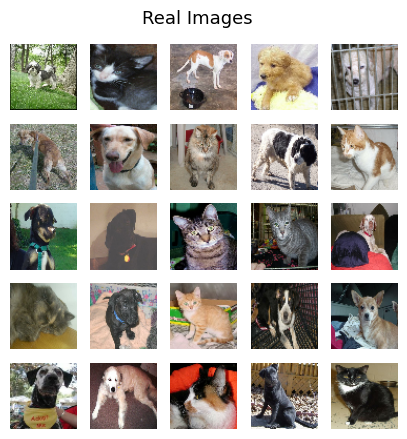
\includegraphics[width=\linewidth]{images/cats_vs_dogs.png}
        \caption{تصاویر مجموعه داده \lr{Cats-vs-Dogs}}
    \end{subfigure}
    \newline
    \begin{subfigure}{0.4\linewidth}
        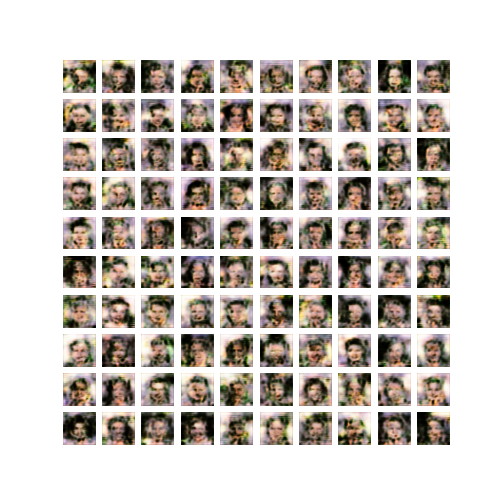
\includegraphics[width=\linewidth]{images/celeb-a_generated.png}
        \caption{تصاویر تولید شده برای مجموعه داده \lr{Celeb-A}}
    \end{subfigure}
    \hfill
    \begin{subfigure}{0.4\linewidth}
        
\includegraphics[width=\linewidth]{images/dcgan/nlayer1/generated_img_30.png}
        \caption{تصاویر تولید شده برای مجموعه داده \lr{Cats-vs-Dogs}}
    \end{subfigure}
    \caption{مقایسه خروجی مدل برای مجموعه داده \lr{Celeb-A} و \lr{Cats-vs-Dogs}}
    \label{celeba}
\end{figure}

\clearpage

\section*{سوال پنج}

راه‌حل‌های پیشنهادی به ترتیب لیست می‌شود.

\begin{itemize}
    \item \textbf{تغییر تابع خطای شبکه مولد}: شبکه مولد در تابع خطایی که در مقاله \lr{GAN} ارائه
    شده است دارای فرمول $\min \log(1-D(G(z)))$ است. اما از آن‌جا که این تابع خطا دارای گرادیان
    میرا است در نتیجه به جای آن از این تابع خطا استفاده می‌کنند: $\max \log(D(G(z)))$.
    \item \textbf{هموارسازی برچسب‌ها}: در این حالت به جای آن که برای داده‌های واقعی برچسب $1$
    و برای داده‌های جعلی برچسب $0$ زده شود، اندکی نویز به آن‌ها اعمال شده و برای داده‌های واقعی برچسبی
    بین $0.7$ تا $1.2$ و برای داده‌های جعلی برچسبی بین $0$ و $0.3$ نسبت داده می‌شود.
    \item \textbf{اضافه‌کردن لایه‌های \lr{dropout} به مدل مولد}: اضافه کردن \lr{dropout} به شبکه مولد باعث
    می‌شود شبکه در هر زمان با بخشی از مدل خود خروجی نهایی را تولید کند. در نهایت با برداشتن این لایه‌های
    \lr{dropout} خروجی نهایی شبکه با استفاده از تمام قدرت شبکه تولید می‌شود که در نتیجه خروجی بهتری را به
    همراه دارد.
    \item \textbf{آموزش بیشتر شبکه دسته‌بند}: در این حالت به جای آن که در هر گام یک مرتبه مدل دسته‌بند
    و در گام دیگر شبکه مولد آموزش ببیند، در هر گام شبکه دسته‌بند چند مرتبه و شبکه مولد یک بار آموزش می‌بیند.
    این کار معمولا زمانی انجام می‌شود که قدرت شبکه دسته‌بند کم است و یا نویز موجود در داده‌های ورودی زیاد
    است. البته این روش همواره نتیجه اثربخشی ندارد.
    \item \textbf{اضافه کردن نویز به تصاویر ورودی}: اضافه کردن نویز به تصاویر ورودی سبب می‌شود کار شبکه
    دسته‌بند سخت‌تر شده و در نتیجه از قدرت آن کاسته شود.
\end{itemize}

\section*{سوال شش}

روش‌های متعادل‌سازی برای یکسان کردن قدرت شبکه‌ دسته‌بند و شبکه مولد استفاده می‌شود. یکی از روش‌های
استفاده شده اضافه‌کردن نویز به تصاویر ورودی است. اضافه‌کردن نویز به تصاویر ورودی باعث می‌شود که
تصاویر ورودی از حالت اولیه خود خارج شده و به تصاویر تولید شده توسط مولد شبیه‌تر شوند. در نتیجه کار مدل
دسته‌بند برای دسته‌بندی تصاویر واقعی از جعلی سخت‌تر می‌شود. در نتیجه همین کار انتظار می‌رود که مدل
مولد فرصت بیشتری برای رشد داشته و در نتیجه کیفیت تصاویر خروجی بهتر شود. البته اگر شدت تصاویر نویز
خیلی زیاد باشد، مدل ‌دسته‌بند نمی‌تواند به خوبی عمل کند و در نتیجه تصاویر تولید شده خوب نخواهند بود.
بنابراین نیاز است که نویز وارد شده بهینه باشد تا قدرت شبکه دسته‌بند به صورت کنترل شده کاهش یابد.

ما ابتدا نتایج حاصل شده برای مدل \lr{FCGAN} را بررسی می‌کنیم.

نویز اعمال شده در این جا نویز نرمال بوده و شدت آن‌ را با استفاده از انحراف معیار کم‌‌وزیاد کرده‌ایم.
در این آزمایش سه مقدار مختلف برای مختلف برای انحراف معیار بررسی شده است: $0.5$، $2$، $5$.
همچنین شبکه با توجه به توضیحات سوال چهار شبکه با یک لایه پنهان بهترین عملکرد را داشته و در نتیجه ما
آن شبکه را در این قسمت انتخاب کرده‌ایم. همان‌طور که مشاهده می‌شود با افزایش شدت نویز تصاویر کم‌رنگ‌تر می‌شوند.
این اتفاق را می‌توان این گونه توجیه کرد که با افزایش نویز عملکرد شبکه دسته‌بند رفته‌رفته کاهش پیدا می‌کند
و در نتیجه مدل مولد نمی‌تواند به خوبی آموزش ببیند.

\begin{figure}[h]
    \begin{subfigure}{0.3\linewidth}
        \includegraphics[width=\linewidth]{images/fcgan/noisy_std0.2/generated_img_01.png}
        \caption{گام اول}
    \end{subfigure}
    \begin{subfigure}{0.3\linewidth}
        \includegraphics[width=\linewidth]{images/fcgan/noisy_std0.2/generated_img_15.png}
        \caption{گام 15ام}
    \end{subfigure}
    \begin{subfigure}{0.3\linewidth}
        
\includegraphics[width=\linewidth]{images/fcgan/noisy_std0.2/generated_img_30.png}
        \caption{گام 30ام}
    \end{subfigure}
    \caption{آموزش شبکه \lr{FCGAN} در طی ۳۰گام\\ نویز اعمال شده $\mathcal{N}(0,0.5)$}
    \label{fcgan_noisy_std0.2}
\end{figure}

\begin{figure}[h]
    \begin{subfigure}{0.3\linewidth}
        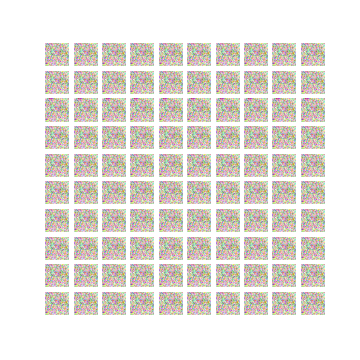
\includegraphics[width=\linewidth]{images/fcgan/noisy_std2.0/generated_img_01.png}
        \caption{گام اول}
    \end{subfigure}
    \begin{subfigure}{0.3\linewidth}
        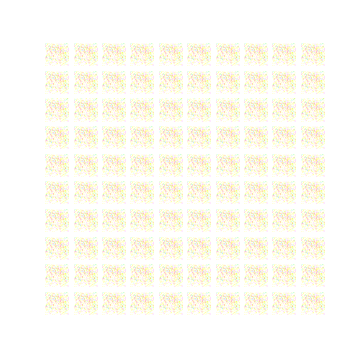
\includegraphics[width=\linewidth]{images/fcgan/noisy_std2.0/generated_img_15.png}
        \caption{گام 15ام}
    \end{subfigure}
    \begin{subfigure}{0.3\linewidth}
        
\includegraphics[width=\linewidth]{images/fcgan/noisy_std2.0/generated_img_30.png}
        \caption{گام 30ام}
    \end{subfigure}
    \caption{آموزش شبکه \lr{FCGAN} در طی ۳۰گام\\ نویز اعمال شده $\mathcal{N}(0,2)$}
    \label{fcgan_noisy_std2.0}
\end{figure}

\begin{figure}[h]
    \begin{subfigure}{0.3\linewidth}
        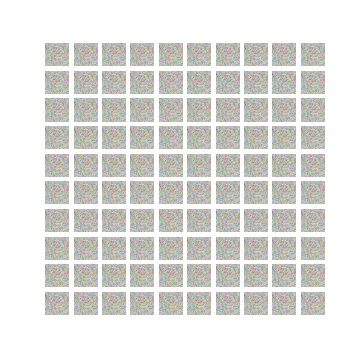
\includegraphics[width=\linewidth]{images/fcgan/noisy_std5.0/generated_img_01.png}
        \caption{گام اول}
    \end{subfigure}
    \begin{subfigure}{0.3\linewidth}
        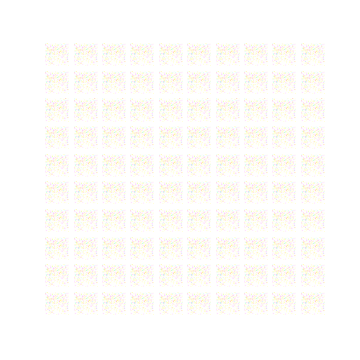
\includegraphics[width=\linewidth]{images/fcgan/noisy_std5.0/generated_img_15.png}
        \caption{گام 15ام}
    \end{subfigure}
    \begin{subfigure}{0.3\linewidth}
        
\includegraphics[width=\linewidth]{images/fcgan/noisy_std5.0/generated_img_30.png}
        \caption{گام 30ام}
    \end{subfigure}
    \caption{آموزش شبکه \lr{FCGAN} در طی ۳۰گام\\ نویز اعمال شده $\mathcal{N}(0,5)$}
    \label{fcgan_noisy_std5.0}
\end{figure}

حال به بررسی نتایج برای مدل \lr{DCGAN} می‌پردازیم.

در این حالت نیز شبکه‌ای که بهترین عملکرد را در سوال ۴ داشته انتخاب شده و مورد بررسی قرار گرفته است.
نویز اعمال شده در این جا نویز اعمال شده چندان روی خروجی تاثیری نگذاشته است و همان‌طور که مشاهده می‌شود
خروجی هر سه حالت با هم مشابه است. دلیل این اتفاق را می‌توان در قدرت کانولوشن دانست. بدین طریق که
حتی با افزایش نویز همچنان شبکه دسته‌بند از قدرت کافی بهره‌مند بوده و می‌توانسته است تصویر واقعی را از جعلی
تشخیص دهد.

\begin{figure}[h]
    \begin{subfigure}{0.3\linewidth}
        \includegraphics[width=\linewidth]{images/dcgan/noisy_std0.2/generated_img_01.png}
        \caption{گام اول}
    \end{subfigure}
    \begin{subfigure}{0.3\linewidth}
        \includegraphics[width=\linewidth]{images/dcgan/noisy_std0.2/generated_img_15.png}
        \caption{گام 15ام}
    \end{subfigure}
    \begin{subfigure}{0.3\linewidth}
        
\includegraphics[width=\linewidth]{images/dcgan/noisy_std0.2/generated_img_30.png}
        \caption{گام 30ام}
    \end{subfigure}
    \caption{آموزش شبکه \lr{DCGAN} در طی ۳۰گام\\ نویز اعمال شده $\mathcal{N}(0,0.5)$}
    \label{dcgan_noisy_std0.2}
\end{figure}

\begin{figure}[h]
    \begin{subfigure}{0.3\linewidth}
        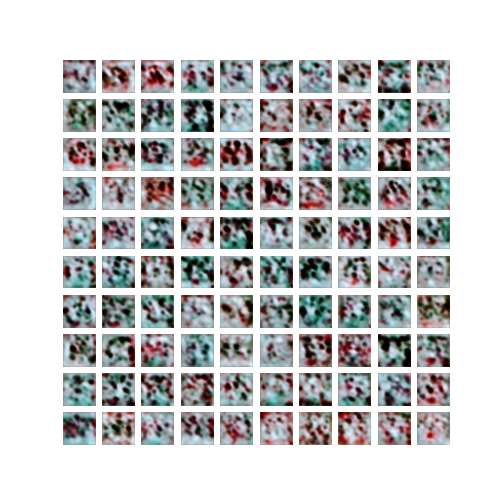
\includegraphics[width=\linewidth]{images/dcgan/noisy_std2.0/generated_img_01.png}
        \caption{گام اول}
    \end{subfigure}
    \begin{subfigure}{0.3\linewidth}
        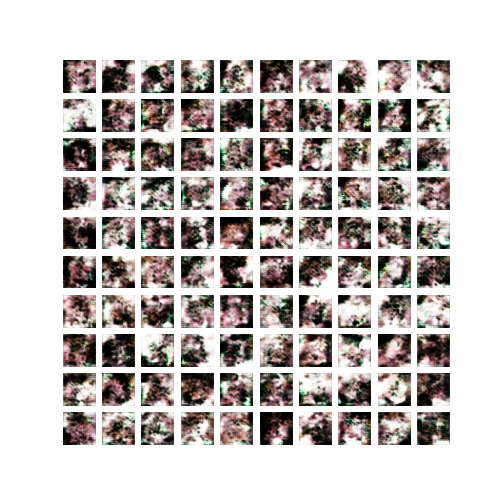
\includegraphics[width=\linewidth]{images/dcgan/noisy_std2.0/generated_img_15.png}
        \caption{گام 15ام}
    \end{subfigure}
    \begin{subfigure}{0.3\linewidth}
        
\includegraphics[width=\linewidth]{images/dcgan/noisy_std2.0/generated_img_30.png}
        \caption{گام 30ام}
    \end{subfigure}
    \caption{آموزش شبکه \lr{DCGAN} در طی ۳۰گام\\ نویز اعمال شده $\mathcal{N}(0,2)$}
    \label{dcgan_noisy_std2.0}
\end{figure}

\begin{figure}[h]
    \begin{subfigure}{0.3\linewidth}
        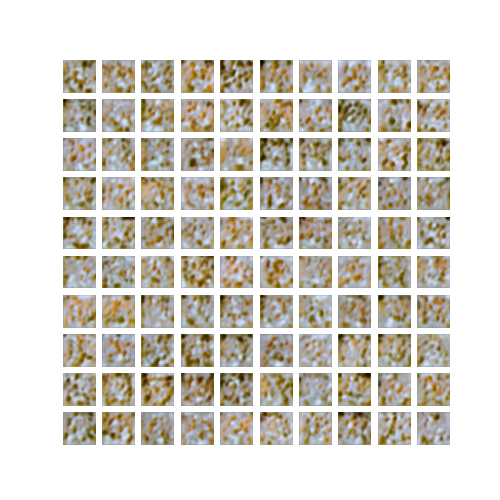
\includegraphics[width=\linewidth]{images/dcgan/noisy_std5.0/generated_img_01.png}
        \caption{گام اول}
    \end{subfigure}
    \begin{subfigure}{0.3\linewidth}
        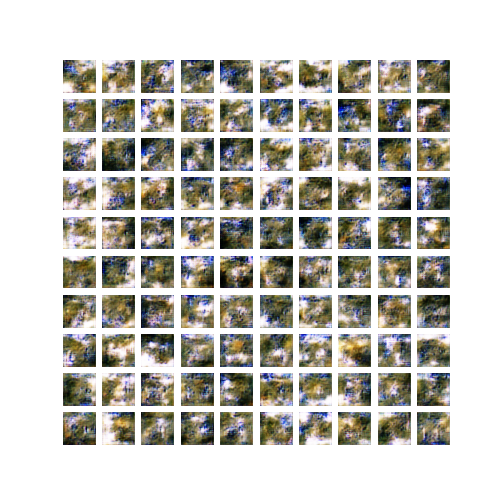
\includegraphics[width=\linewidth]{images/dcgan/noisy_std5.0/generated_img_15.png}
        \caption{گام 15ام}
    \end{subfigure}
    \begin{subfigure}{0.3\linewidth}
        
\includegraphics[width=\linewidth]{images/dcgan/noisy_std5.0/generated_img_30.png}
        \caption{گام 30ام}
    \end{subfigure}
    \caption{آموزش شبکه \lr{DCGAN} در طی ۳۰گام\\ نویز اعمال شده $\mathcal{N}(0,5)$}
    \label{dcgan_noisy_std5.0}
\end{figure}

\section*{سوال هفت}

با توجه به نتایجی که تا به این جا ارائه شد شبکه \lr{DCGAN} عملکرد بسیار بهتری نسبت به شبکه \lr{FCGAN}
دارد. علت این برتری در استفاده از کانوولوشن است. شبکه \lr{DCGAN} می‌تواند برای تولید خروجی‌ها و همچنین
دسته‌بندی داده‌های واقعی از جعلی از کانولوشن استفاده کند در حالی که شبکه \lr{FCGAN} باید از لایه‌های متراکم
استفاده کند. کانولوشن بنا به ماهیتی که دارد می‌تواند ویژگی‌های بسیار بهتری از داده‌ها را تولید کند.
این ویژگی‌ها باعث می‌شود شبکه مولد با استفاده از آن‌ها بتواند خروجی نهایی واقع‌گرایانه‌تری داشته باشد
و در نتیجه نسبت به شبکه مولد \lr{FCGAN} بهتر عمل کند.

\section*{سوال هشت}

تصاویر در قسمت‌های مختلف سوال‌های قبلی نمایش داده شده است. به طور مشخص برای شبکه \lr{DCGAN} شکل
\ref{dcgan_nlayer1} و برای شبکه \lr{FCGAN} شبکه شکل \ref{fcgan_nlayer1} خروجی بهتری را برای شبکه‌ها
ارائه داده‌اند.

\end{document}